\section{Application to NASA CRM} \label{sec:mf_gp_nasa_crm}

To provide more quantitative applications of the RANS UQ methodology, we demonstrate its inclusion in the multi-fidelity GP framework. To showcase the predictive capabilities of the multi-fidelity GP framework, the CFD data is augmented with both low-fidelity simulations, using the Athena Vortex Lattice (AVL) code \cite{drela2008athena}, and high-fidelity experimental data, from the wind tunnel campaigns \cite{rivers_further_2012,rivers_experimental_2010} used in the preceding section. For the vortex-lattice simulations, the uncertainty information is provided by subject matter experts (industry users and academics), while for the experimental data, the uncertainty intervals used are those described in the wind-tunnel campaign reports. 

For the ease of illustration, $C_L$, $C_D$, and $C_m$ are initially considered one-dimensional functions of $\alpha$ ($m = 1$). The methodology described earlier in Section \ref{sec:mf_modeling} is generally applicable to functions of many variables. Aerodynamic databases are often multi-dimensional functions, often with a maximum of 5 input variables (angle of attack, side-slip angle, Mach number, altitude, and dynamic pressure). Multi-dimensional, multi-fidelity databases are explored towards the end of this section. 

The results of the multi-fidelity modeling with one input variable ($\alpha$) are presented in Figures \ref{fig:cl_alpha_mf} -- \ref{fig:cm_alpha_mf}. For each figure, the solid black line represents the mean predicted by the GP and the grey area represents the $\pm 2\sigma$ interval as predicted by the GP. The left column of figures shows purely the AVL data and a single-fidelity GP fit on that data. In the middle we introduce the SU2 RANS CFD data with uncertainty bounds informed by the RANS UQ methodology, and show the two-fidelity GP fit. On the right we introduce a limited set of wind tunnel data points to inform the highest fidelity, and show the resulting three-fidelity fit. For each QoI the build-up of the database is shown, and the distribution of data points across fidelity levels is shown in Table \ref{table:data_points}.

\begin{table}
\centering
    \captionsetup{justification=centering}
    \caption{Number of data points of each fidelity that are used to create Figures \ref{fig:cl_alpha_mf}-\ref{fig:cm_alpha_mf}.} 
    \begin{tabular}{|c|c|}
        \hline
        Data Source & Data Points \\ \hline \hline
        Low Fidelity (AVL) & 23 \\ \hline
        Medium Fidelity (CFD) & 11 \\ \hline 
        High Fidelity (Wind Tunnel) & 5 \\ \hline 
    \end{tabular}
    \label{table:data_points}
\end{table}

In the three-fidelity fits of Figures \ref{fig:cl_alpha_mf}(c) -- \ref{fig:cm_alpha_mf}(c) the wind tunnel data points are evenly spread across the domain of interest, $-2^\circ \leq \alpha \leq 12^\circ$. These data points also have uncertainties associated with them, but these are very small and cannot be seen on this scale in the figures. For the second and third column of figures, the mean and standard deviation predictions are made by the multi-fidelity GP methodology from Section \ref{sec:mf_modeling}. 

\begin{figure}
    \centering
    \begin{subfigure}[Single fidelity fit.] {
        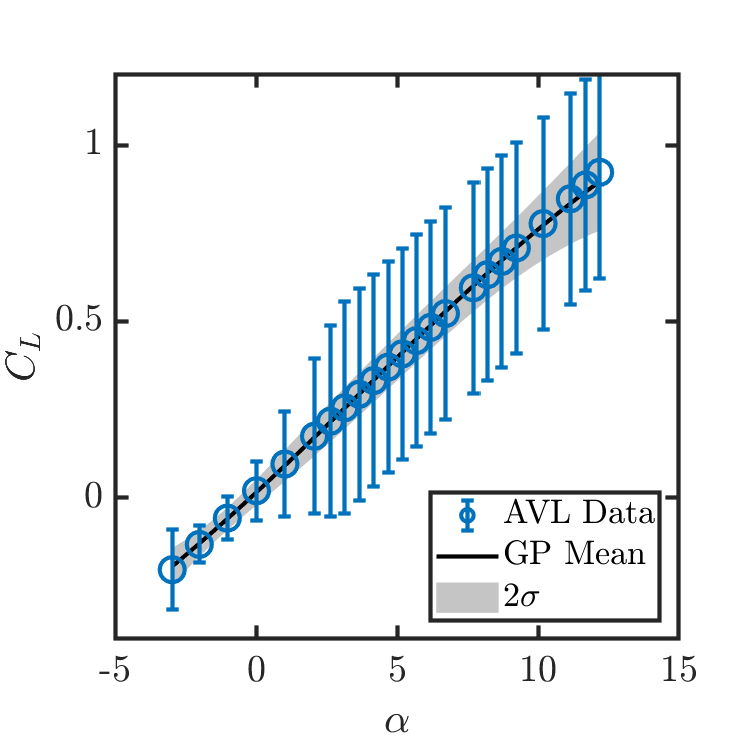
\includegraphics[width=.31\textwidth]{code/image_gen/nasa_crm/images/cl_1f.png} }
    \end{subfigure}
    \hfill
    \begin{subfigure}[Two-fidelity fit.]{
        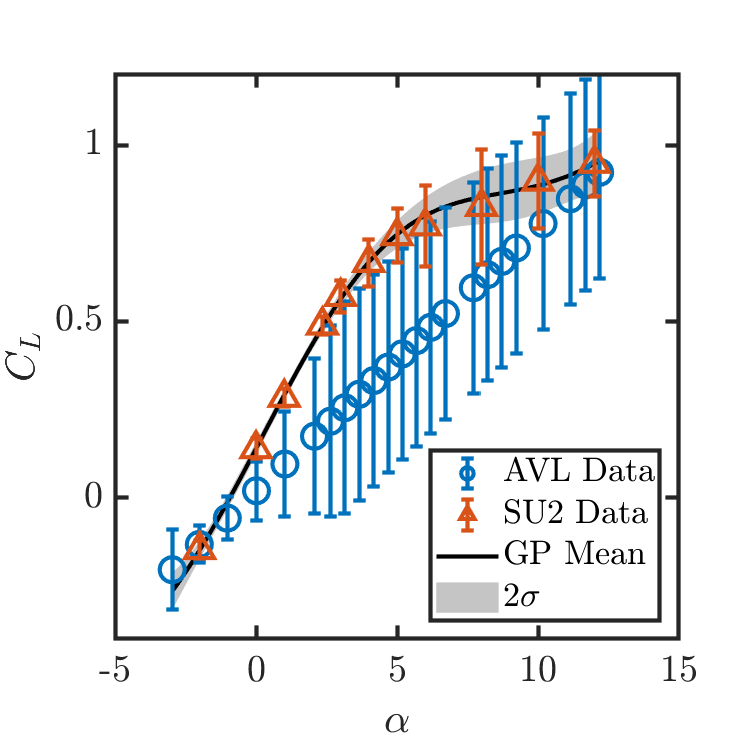
\includegraphics[width=.31\textwidth]{code/image_gen/nasa_crm/images/cl_2f.png} 
    }
    \end{subfigure}
    \hfill
    \begin{subfigure}[Three-fidelity fit.]{
        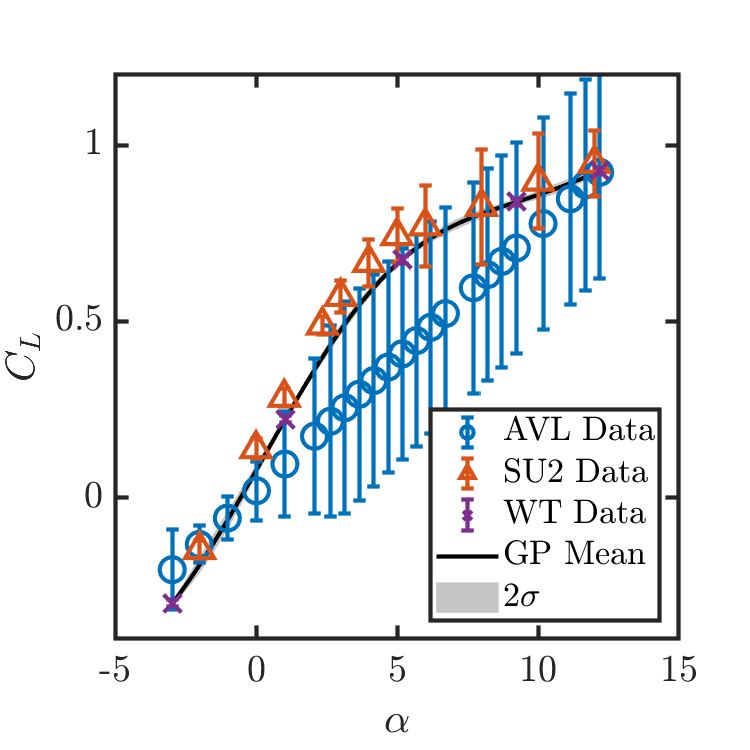
\includegraphics[width=.31\textwidth]{code/image_gen/nasa_crm/images/cl_3f.png} 
    }
    \end{subfigure}
    \caption{$C_L$ vs $\alpha$ for the NASA CRM, using data from multiple sources of varying fidelity.\label{fig:cl_alpha_mf}}
    \hfill
    \centering
    \begin{subfigure}[Single fidelity fit.] {
        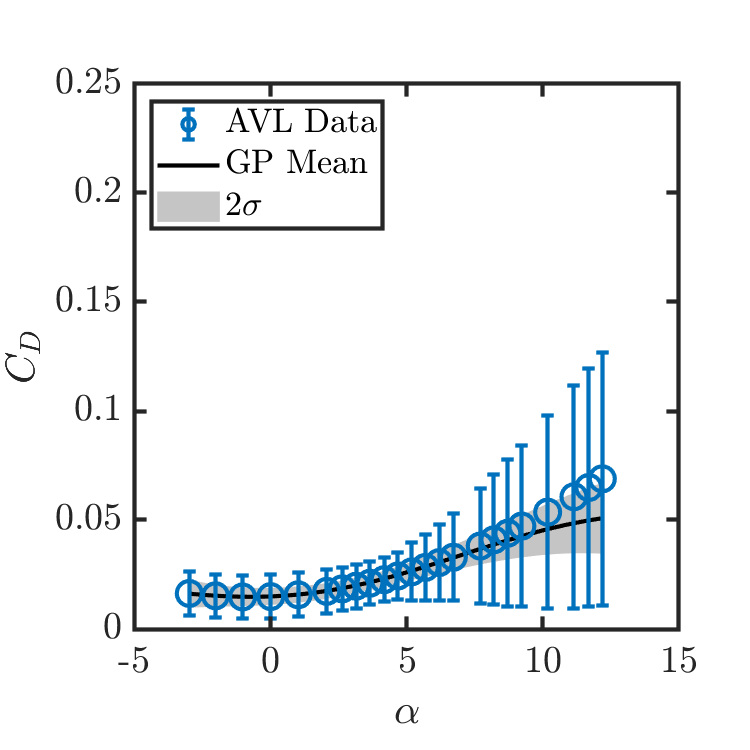
\includegraphics[width=.31\textwidth]{code/image_gen/nasa_crm/images/cd_1f.png} }
    \end{subfigure}
    \hfill
    \begin{subfigure}[Two-fidelity fit.]{
        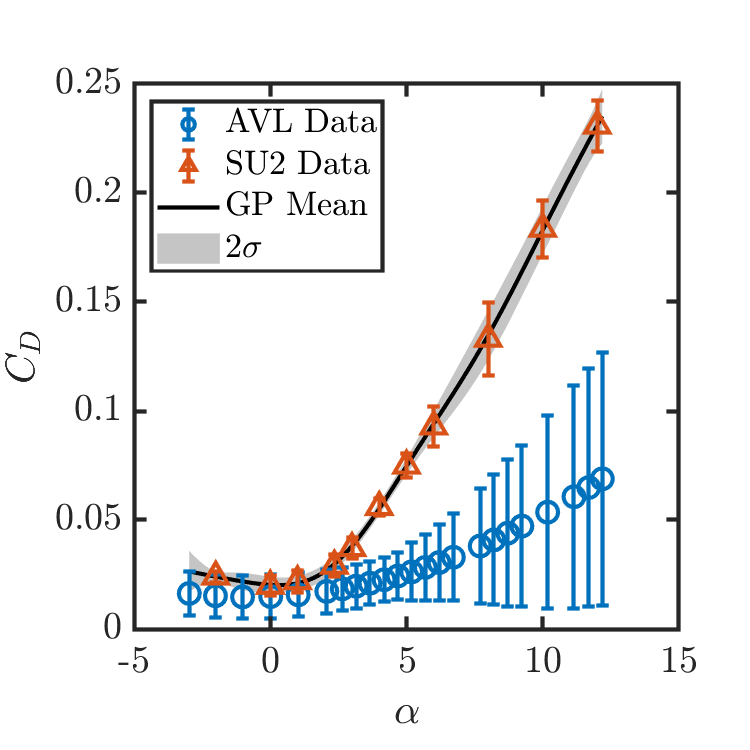
\includegraphics[width=.31\textwidth]{code/image_gen/nasa_crm/images/cd_2f.png} 
    }
    \end{subfigure}
    \hfill
    \begin{subfigure}[Three-fidelity fit.]{
        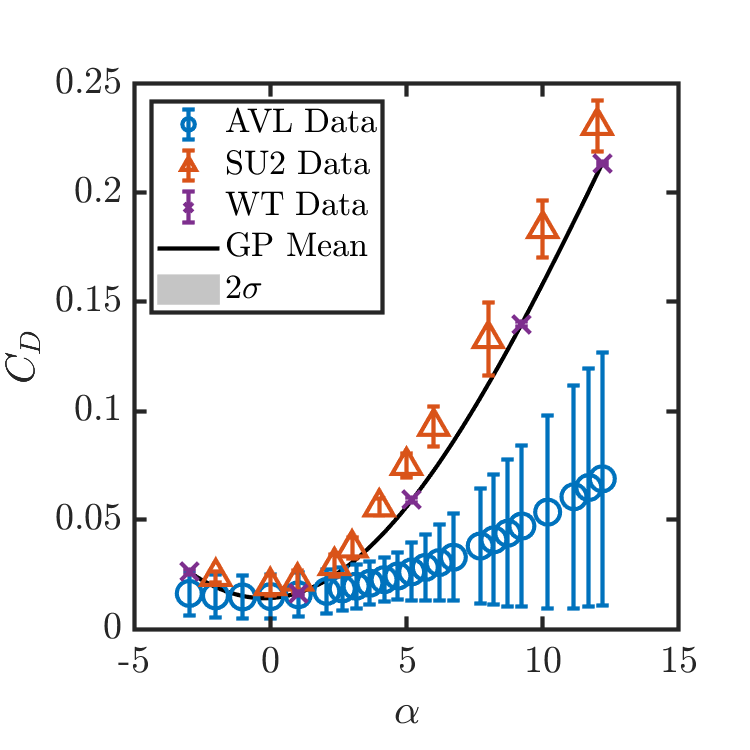
\includegraphics[width=.31\textwidth]{code/image_gen/nasa_crm/images/cd_3f.png} 
    }
    \end{subfigure}
    \caption{$C_D$ vs $\alpha$ for the NASA CRM, using data from multiple sources of varying fidelity.\label{fig:cd_alpha_mf}}
    \hfill
    \centering
    \begin{subfigure}[Single fidelity fit.] {
        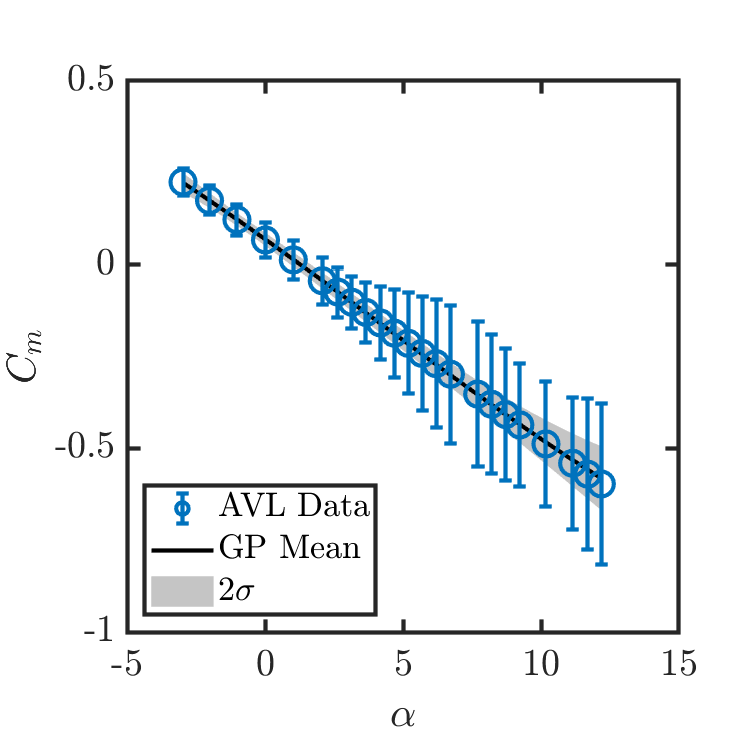
\includegraphics[width=.31\textwidth]{code/image_gen/nasa_crm/images/cm_1f.png} }
    \end{subfigure}
    \hfill
    \begin{subfigure}[Two-fidelity fit.]{
        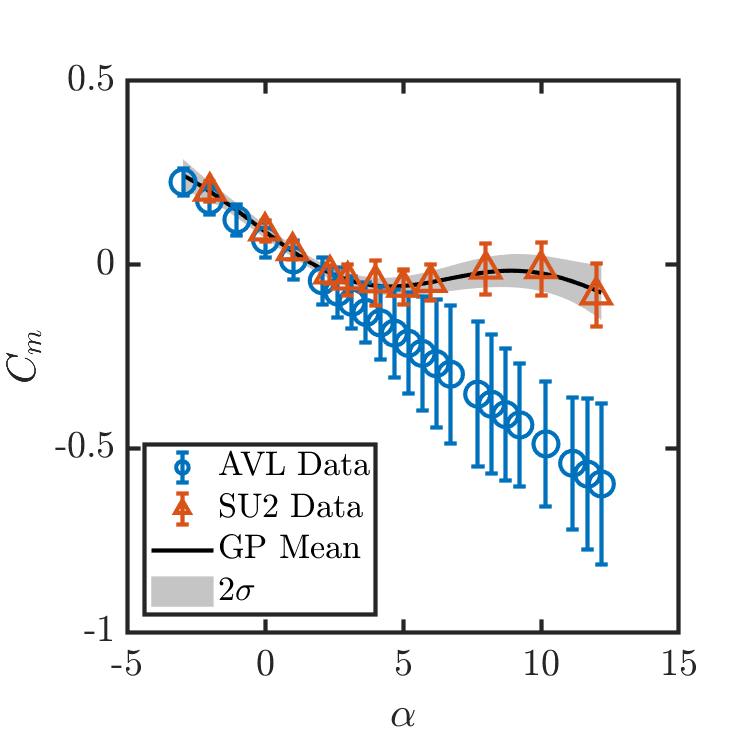
\includegraphics[width=.31\textwidth]{code/image_gen/nasa_crm/images/cm_2f.png} 
    }
    \end{subfigure}
    \hfill
    \begin{subfigure}[Three-fidelity fit.]{
        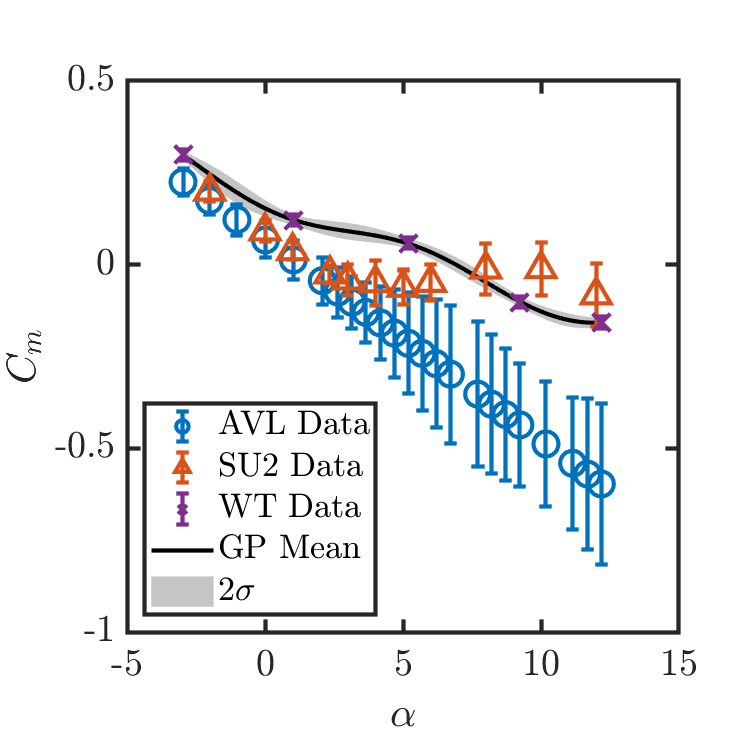
\includegraphics[width=.31\textwidth]{code/image_gen/nasa_crm/images/cm_3f.png} 
    }
    \end{subfigure}
    \caption{$C_m$ vs $\alpha$ for the NASA CRM, using data from multiple sources of varying fidelity.\label{fig:cm_alpha_mf}}
\end{figure}

The multi-fidelity GPs are able to learn the biases between the different fidelity levels and provide predictions that fit very well with the highest fidelity. To show the benefit of using multi-fidelity data vs. using only high-fidelity data points, the root-mean-square error (RMSE) for both cases and for each QoI is presented in Figure \ref{fig:mf_vs_hf}. The error is calculated using the $N$ highest-fidelity data points that aren't used in training the model as:

\begin{equation}\label{equ:rmse}
    RMSE = \sqrt{\frac{\sum_{i=1}^{N}\left ( \mu_{s,i} - y_{s,i} \right )^2}{N}},
\end{equation}
where $y_{s,i}$ is the $i$-th data point of the highest ($s$) fidelity, and $\mu_{s,i}$ is the highest-fidelity prediction from the GP at the same input conditions.  

Since the QoIs are simple functions of $\alpha$, not many high-fidelity data points are required to accurately capture the functional dependence. The differences between the prediction accuracy for a single- vs. multi-fidelity fit is not significant. Nonetheless, the trends are what would be expected. When high-fidelity data is scarce, the multi-fidelity predictions perform better for all QoIs since the low-fidelity data helps provide general trends that are learned by the multi-fidelity GP. As the number of high-fidelity data points increases, the RMSEs converge since there is enough data for both fits to accurately reproduce the functional dependence. When the domain is very well covered by high-fidelity data, the single-fidelity fits can do marginally better since the low-fidelity data (in the multi-fidelity fits) doesn't provide any useful information and can serve to introduce noise in the predictions.

\begin{figure}
    \centering
    \begin{subfigure}[RMSE for $C_L$ vs. $\alpha$.] {
        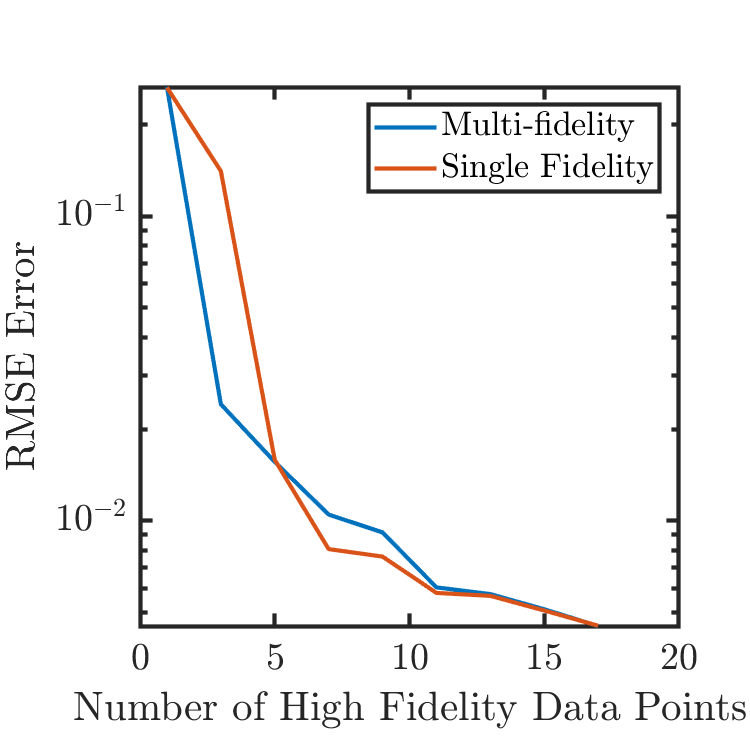
\includegraphics[width=.31\textwidth]{code/image_gen/nasa_crm/images/cl_rsme_comp.png} }
    \end{subfigure}
    \hfill
    \begin{subfigure}[RMSE for $C_D$ vs. $\alpha$.]{
        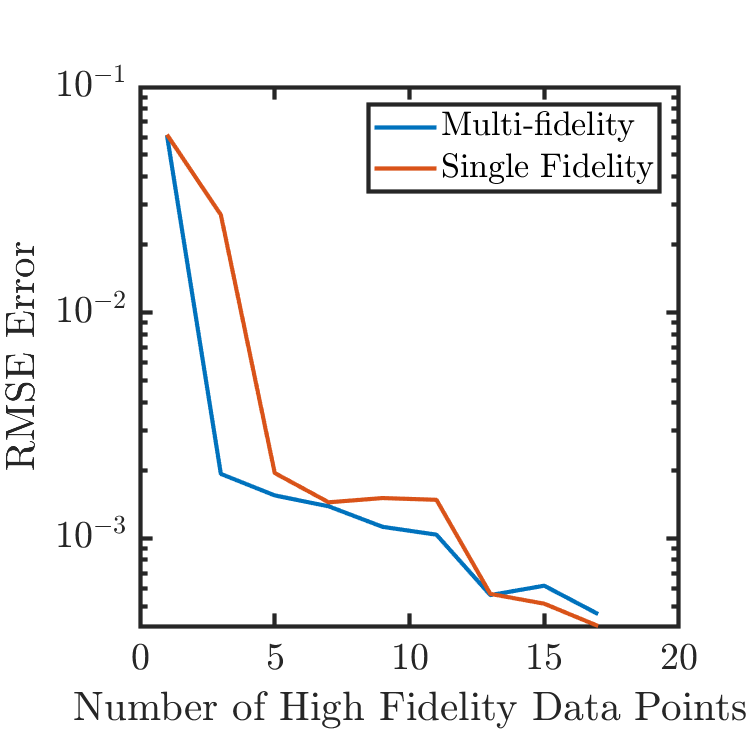
\includegraphics[width=.31\textwidth]{code/image_gen/nasa_crm/images/cd_rsme_comp.png} 
    }
    \end{subfigure}
    \hfill
    \begin{subfigure}[RMSE for $C_m$ vs. $\alpha$.]{
        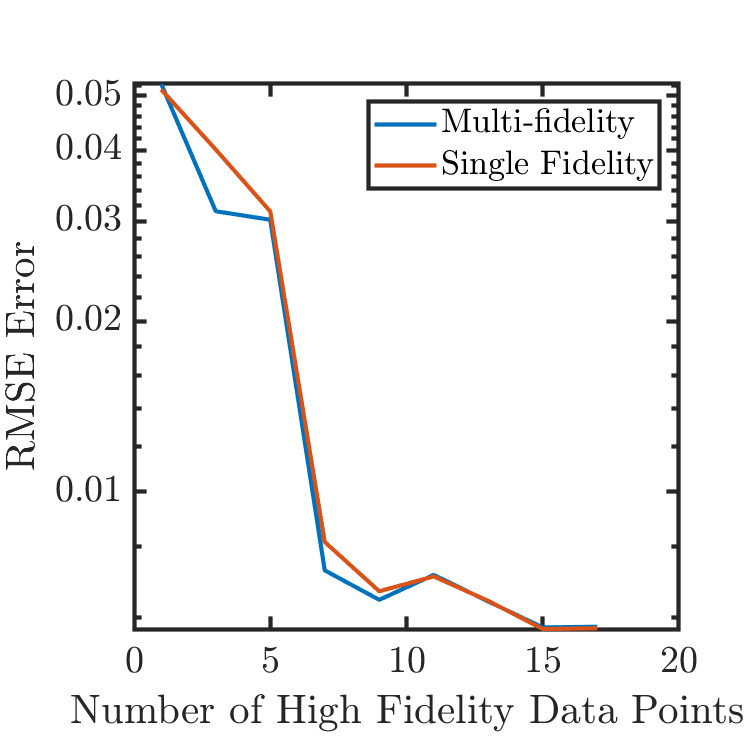
\includegraphics[width=.31\textwidth]{code/image_gen/nasa_crm/images/cm_rsme_comp.png} 
    }
    \end{subfigure}
    \caption{Root Mean Square error when using three-fidelity data vs. using only high-fidelity data points.\label{fig:mf_vs_hf}}
\end{figure}

Another strength of this multi-fidelity GP methodology is apparent when the high-fidelity data is localized to a certain part of the domain. Such a situation might arise if resources are limited and it is not feasible to perform high-fidelity evaluations over the entire domain of interest. It might also be the case that the lower-fidelity simulations are fairly accurate in a certain part of the domain and, consequently, introduce smaller uncertainties in these regions of the domain. For the NASA CRM it is mentioned in Section \ref{sec:crm_rans_uq} that at low angles of attack, where the flow remains attached to the aircraft, RANS CFD simulations are quite successful at predicting performance metrics. This is evidenced by the smaller uncertainty bounds predicted by the RANS UQ methodology in Figure \ref{fig:crm_su2_uq} at $\alpha < 5^\circ$. In this case, an engineer might conclude that highest-fidelity evaluations are not necessary at $\alpha < 5^\circ$ and that sufficient accuracy can be achieved with just the lower-fidelity sources. 

To simulate such a situation, a multi-fidelity GP is created that uses AVL and SU2 data that spans the entire domain of interest, but uses wind tunnel evaluations only at high angles of attack $(\alpha > 5^\circ)$. This is a manufactured situation where we choose to ignore some of the wind tunnel data to illustrate the ability of the multi-fidelity GP framework to perform reliably without high-fidelity information that spans the domain of interest. Figure \ref{fig:mf_partial} presents the predictions made by a three-fidelity GP trained on AVL, SU2, and wind tunnel data (left column), and a single-fidelity GP trained on just the wind tunnel data (middle column). The wind tunnel data used to train the models is restricted to high angles of attack, but the unused wind tunnel data is also included in the plots to discern the quality of the predictions. The right column presents the RMSE of the predictions made by the single- and multi-fidelity GPs when using localized high-fidelity data. The case that is shown in the left and middle columns, is highlighted in this error comparison. From the RMSE comparison, it is clear that having accurate low-fidelity data at low angles of attack informs the GP prediction in that region, and allows it to follow the trend of the physical phenomena more accurately than when only the localized high-fidelity data is used. 

\begin{figure}
    \centering
    \begin{subfigure}[$C_L vs. \alpha$: Three-fidelity fit.] {
        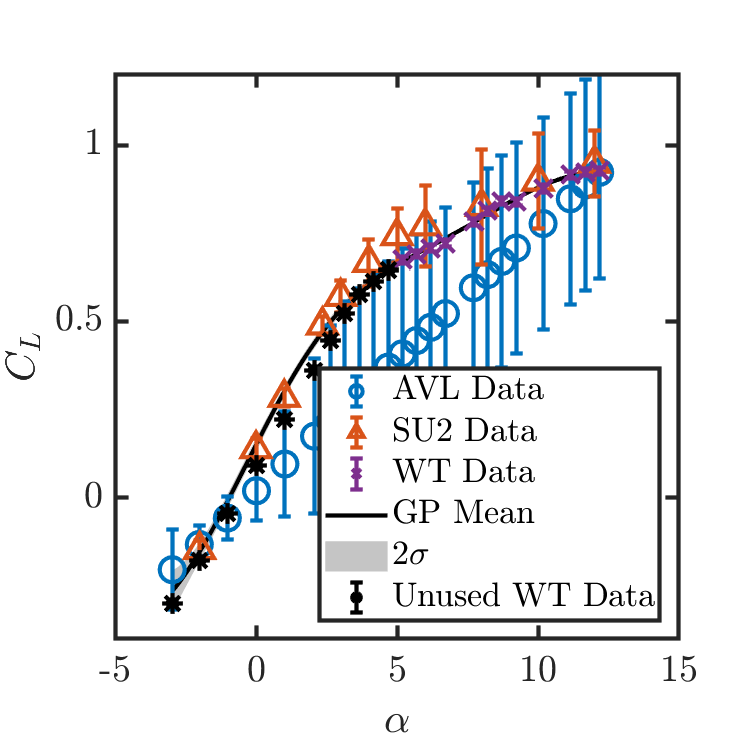
\includegraphics[width=.31\textwidth]{code/image_gen/nasa_crm/images/cl_3f_partial.png} }
    \end{subfigure}
    \begin{subfigure}[$C_L vs. \alpha$: Single fidelity fit.]{
        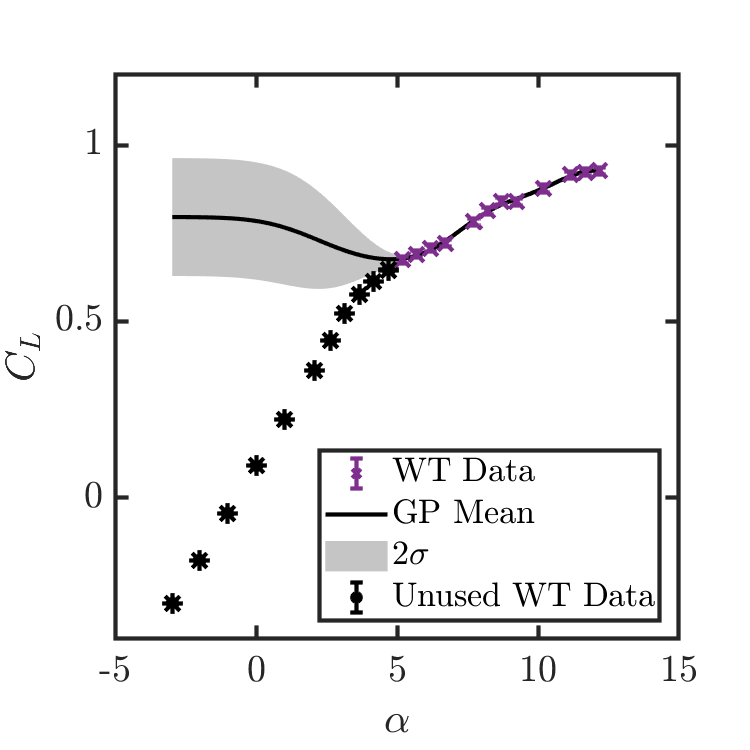
\includegraphics[width=.31\textwidth]{code/image_gen/nasa_crm/images/cl_hf_partial.png} 
    }
    \end{subfigure}
    \hfill
    \begin{subfigure}[$C_L vs. \alpha$: RMSE trends when data is added sequentially from high to low values of $\alpha$.]{
        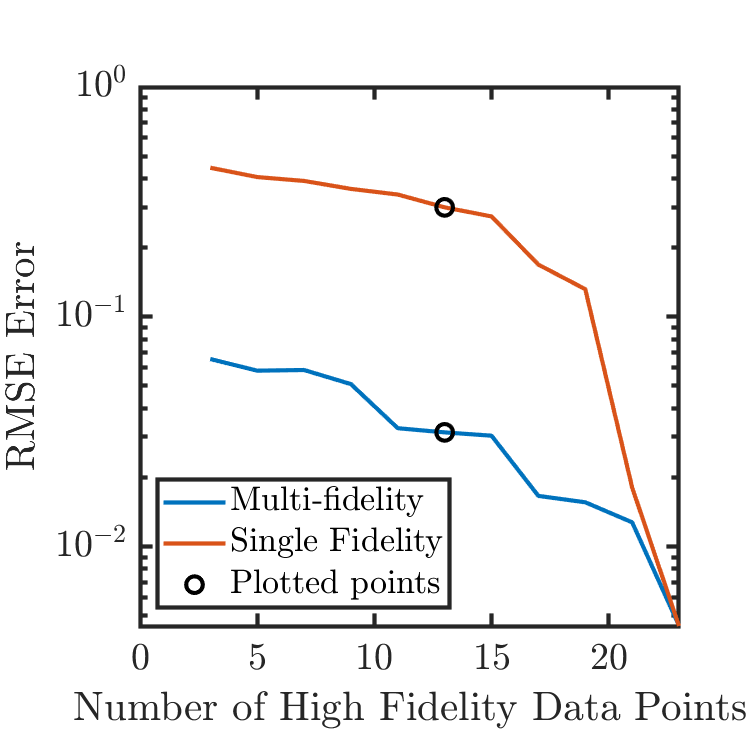
\includegraphics[width=.31\textwidth]{code/image_gen/nasa_crm/images/cl_rsme_local_comp.png} 
    }
    \end{subfigure}

    \begin{subfigure}[$C_D vs. \alpha$: Three-fidelity fit.] {
        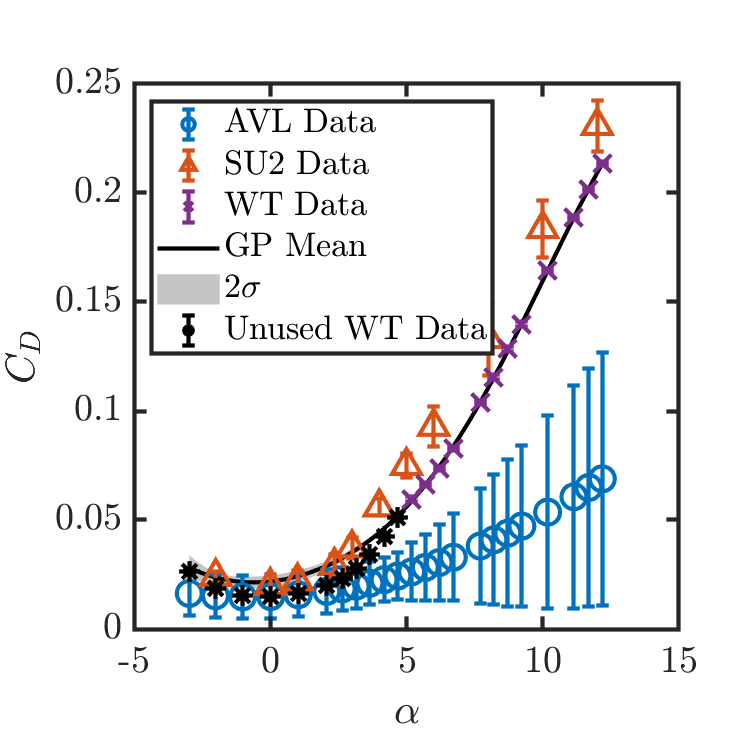
\includegraphics[width=.31\textwidth]{code/image_gen/nasa_crm/images/cd_3f_partial.png} }
    \end{subfigure}
    \begin{subfigure}[$C_D vs. \alpha$: Single fidelity fit.]{
        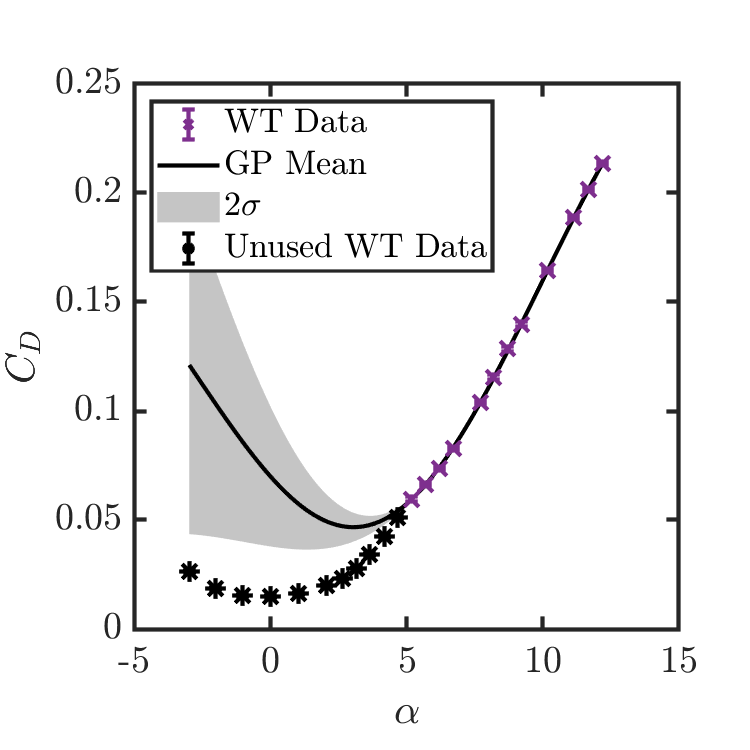
\includegraphics[width=.31\textwidth]{code/image_gen/nasa_crm/images/cd_hf_partial.png} 
    }
    \end{subfigure}
    \hfill
    \begin{subfigure}[$C_D vs. \alpha$: RMSE trends when data is added sequentially from high to low values of $\alpha$.]{
        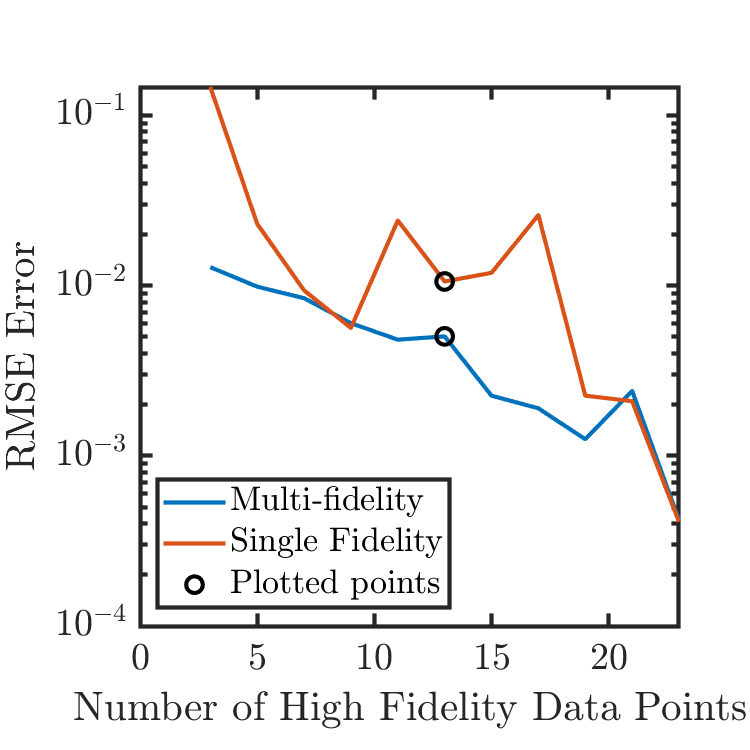
\includegraphics[width=.31\textwidth]{code/image_gen/nasa_crm/images/cd_rsme_local_comp.png} 
    }
    \end{subfigure}

    \begin{subfigure}[$C_m vs. \alpha$: Three-fidelity fit.] {
        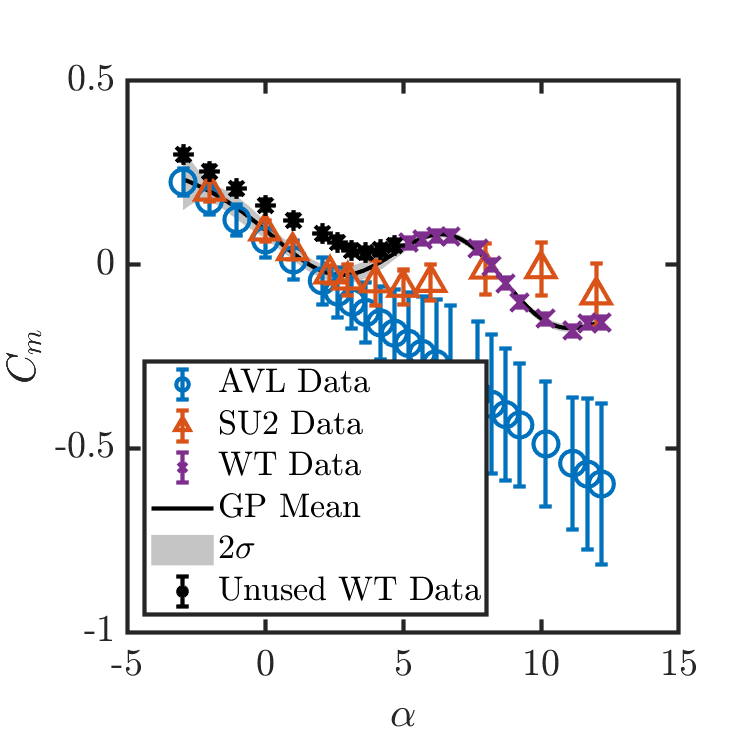
\includegraphics[width=.31\textwidth]{code/image_gen/nasa_crm/images/cm_3f_partial.png} }
    \end{subfigure}
    \begin{subfigure}[$C_m vs. \alpha$: Single fidelity fit.]{
        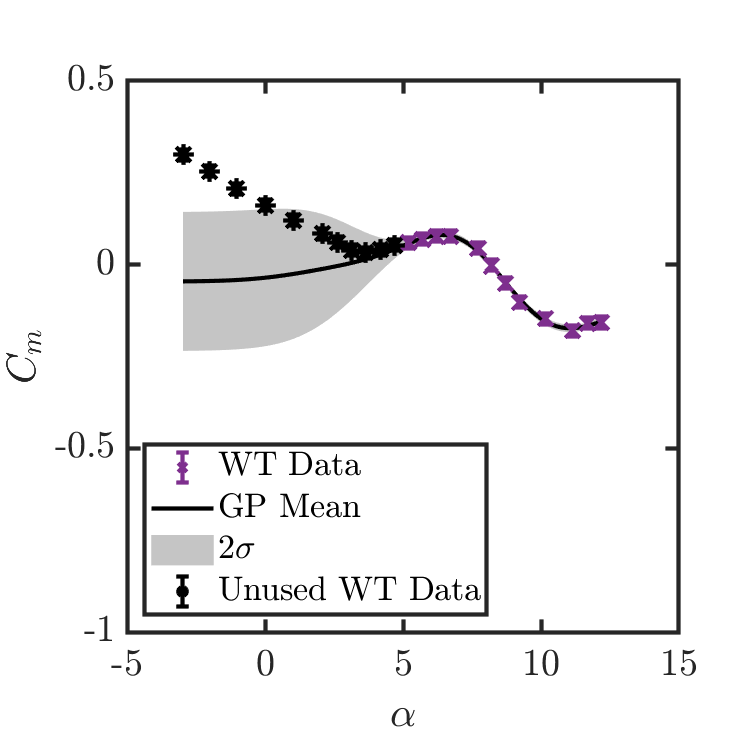
\includegraphics[width=.31\textwidth]{code/image_gen/nasa_crm/images/cm_hf_partial.png} 
    }
    \end{subfigure}
    \hfill
    \begin{subfigure}[$C_m vs. \alpha$: RMSE trends when data is added sequentially from high to low values of $\alpha$.]{
        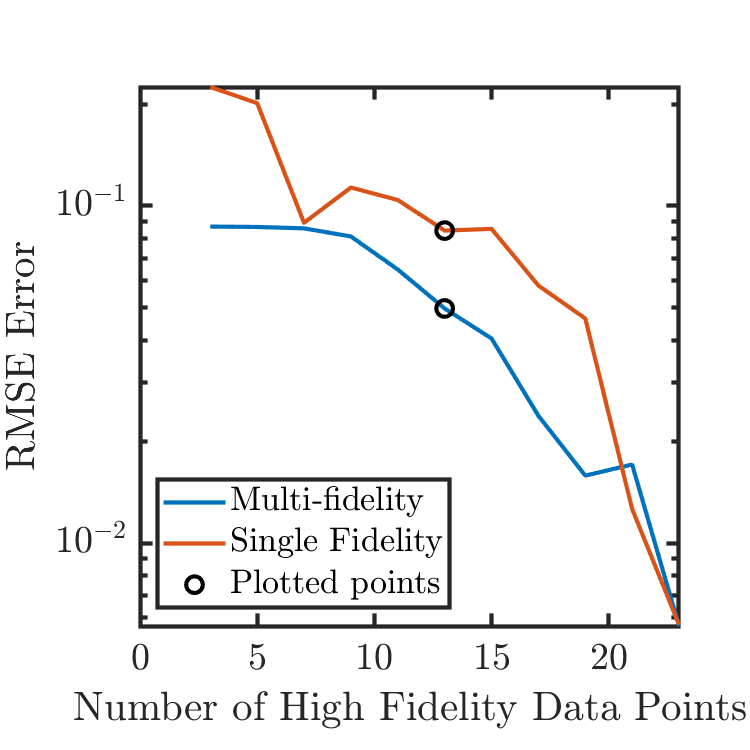
\includegraphics[width=.31\textwidth]{code/image_gen/nasa_crm/images/cm_rsme_local_comp.png} 
    }
    \end{subfigure}
    
    \caption{Showcasing the superior predictive capability of multi-fidelity data fusion when high-fidelity data is localized in the design space. The left column represents the multi-fidelity GP formulation result, while the middle column shows the results for the single-fidelity formulation. The right column shows the RMSE error trends when high-fidelity data is localized. The black circles correspond to the specific case shown in the left and middle columns. \label{fig:mf_partial}}
    
\end{figure}

To explore the performance of the multi-fidelity predictive capability in multiple dimensions, the same aerodynamic coefficients from before ($C_L$, $C_D$, and $C_m$) are considered functions of both $\alpha$ and Mach number. Two sources of information, AVL simulations and wind tunnel data, are used to create two-fidelity, two-dimensional GPs. Visualizing the GP predictions in two dimensions is difficult but the results for $C_L$ are shown in Figure \ref{fig:2d_2f_cl_data}. Figure \ref{fig:cl_2d_2f_points} shows the two-fidelity data sets that are used to train the multi-fidelity GP. Figure \ref{fig:cl_2d_2f_surf} shows the surfaces that represent the mean (as a contoured solid surface), and $2\sigma$ interval estimates (as translucent surfaces sandwiching the mean prediction). The difference between the mean and intervals is hard to discern at that scale. Figure \ref{fig:cl_2d_2f_surf_zoom} focuses in on the high-angle of attack (and low Mach number) area when the uncertainties are larger, to show the different surfaces clearly. To show a one-dimensional representation of the data, a slice spanning the two dimensions is taken (shown in red). The mean and $2\sigma$ intervals along that slice are plotted in Figure \ref{fig:cl_2d_2f_sample}, along with some deterministic samples of the GP (multi-colored lines) that show how they might vary spatially. Again since uncertainties are small, an inset focuses on the high-angle of attack (and low Mach number) area of the domain where the individual samples can be recognized.

\begin{figure}
    \centering
    \begin{subfigure}[AVL and wind tunnel data points.] {
        \label{fig:cl_2d_2f_points}
        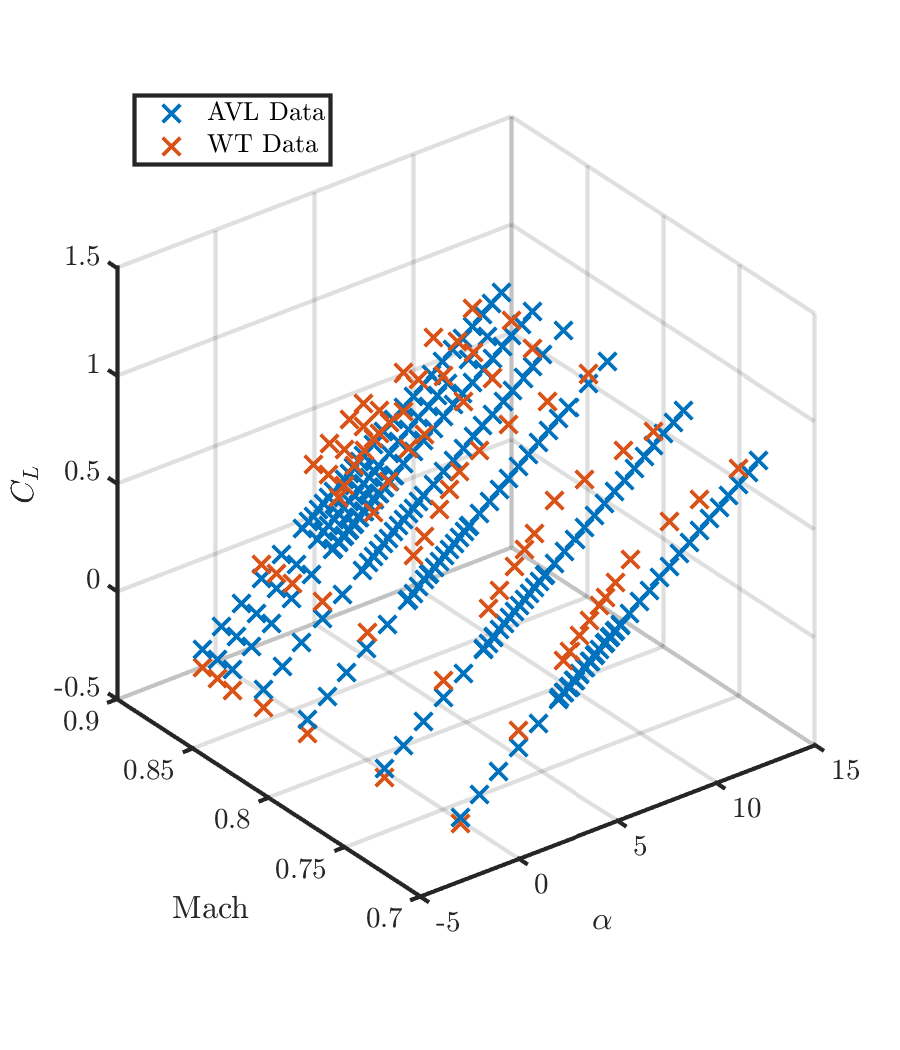
\includegraphics[trim=0 0 0 0, clip, width=.45\textwidth]{code/image_gen/nasa_crm/images/cl_2d_2f_points.png} }
    \end{subfigure}
    \hfill
    \begin{subfigure}[Surfaces representing mean and $2\sigma$ predictions from GP. Red slice shows one-dimensional location for sampling the GP which is shown in \subref{fig:cl_2d_2f_sample}.]{
        \label{fig:cl_2d_2f_surf}
        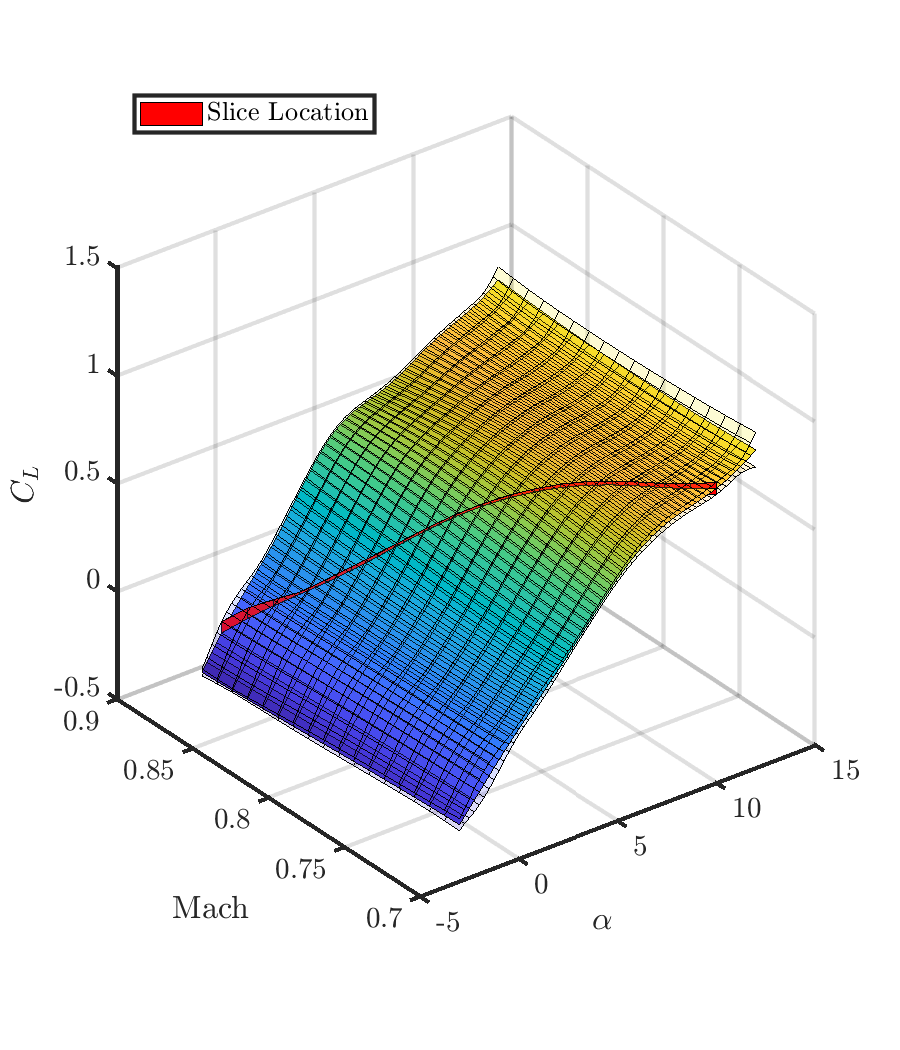
\includegraphics[trim=0 0 0 0, clip, width=.45\textwidth]{code/image_gen/nasa_crm/images/cl_2d_2f_surf.png} 
    }
    \end{subfigure}
    \hfill
    \begin{subfigure}[Zoomed in view of surfaces in \subref{fig:cl_2d_2f_surf} at high angles of attack (and lower Mach number). The mean and $2\sigma$ predictions interval surfaces are more discernible at this scale.]{
        \label{fig:cl_2d_2f_surf_zoom}
        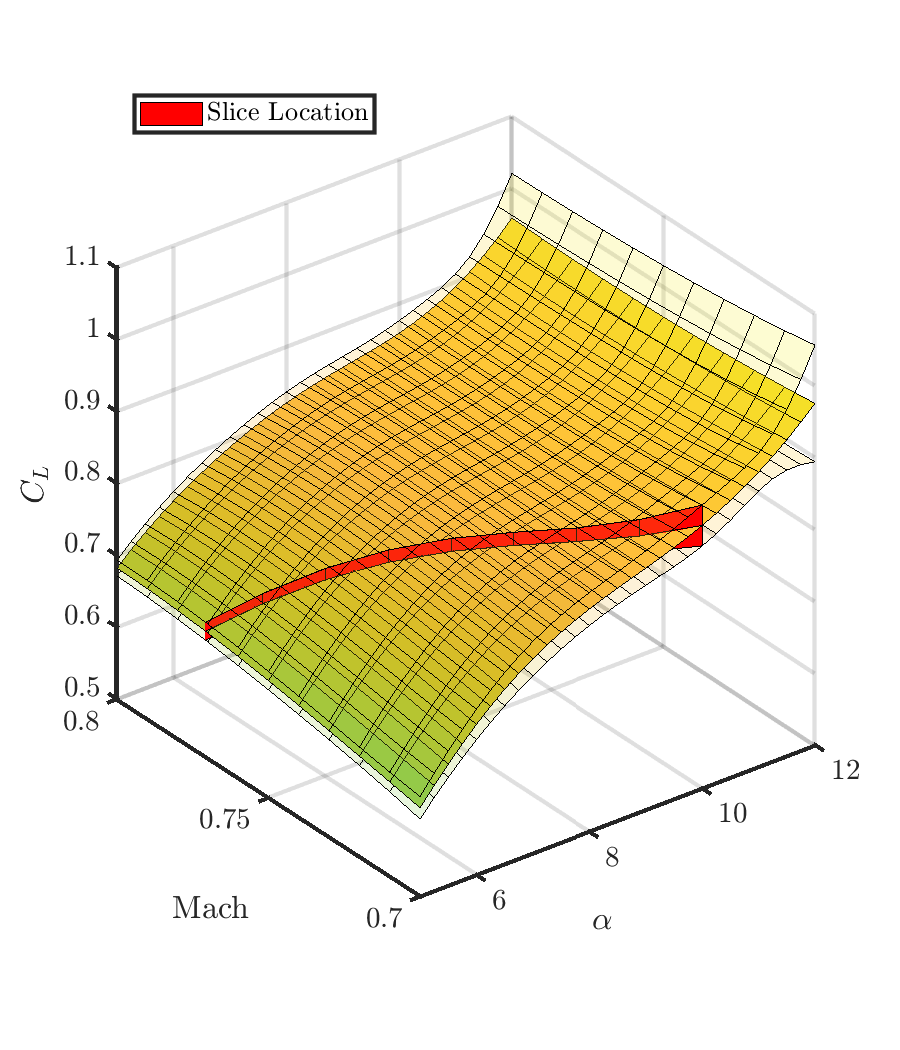
\includegraphics[trim=0 0 0 0, clip, width=.45\textwidth]{code/image_gen/nasa_crm/images/cl_2d_2f_surf_zoom.png} 
    }
    \end{subfigure}
    \hfill
    \begin{subfigure}[One-dimensional representation of mean and $2\sigma$ estimates at slice location shown in \subref{fig:cl_2d_2f_surf}. Multiple samples (colored lines) of the GP are also overlaid to show examples of deterministic sampling. Inset plot focuses in on high angles of attack.]{
        \label{fig:cl_2d_2f_sample}
        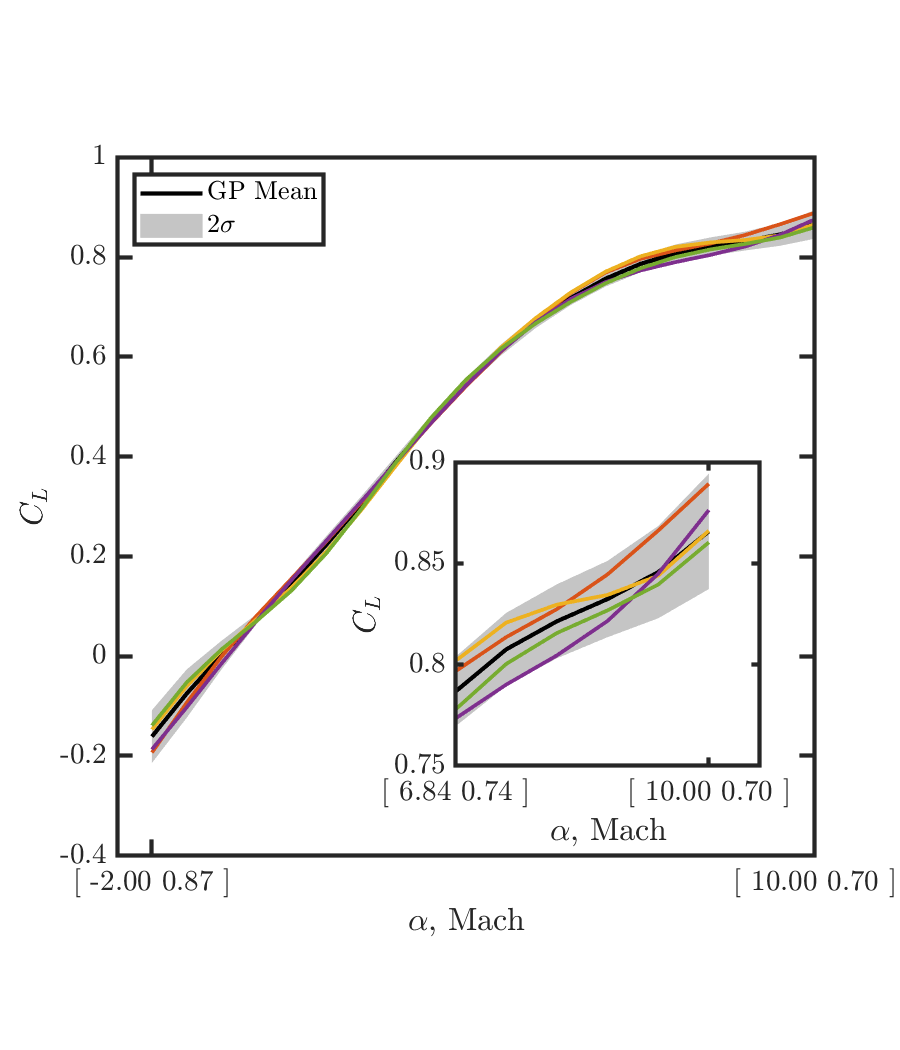
\includegraphics[trim=0 0 0 0, clip, width=.45\textwidth]{code/image_gen/nasa_crm/images/cl_2d_2f_sample.png} 
    }
    \end{subfigure}
    \caption{Two-dimensional representation of $C_L$ as a function of $\alpha$ and Mach number.\label{fig:2d_2f_cl_data}}
\end{figure}

Predictions from the two-fidelity GPs are compared to those made from single-fidelity GPs that use only the wind tunnel data. The change in the root-mean-square-error (Equation \eqref{equ:rmse}) is shown in Fig \ref{fig:2d_mf_vs_hf}. When trying to represent two-dimensional functions, the multi-fidelity fit retains its advantage for longer, with the single-fidelity fit taking $\approx 50$ high-fidelity data points to achieve similar accuracy. If the number of high-fidelity points is increased beyond that, the two fits behave identically. For these results, the high-fidelity data was spread evenly across the domain of interest: $-2^\circ \leq \alpha \leq 12^\circ$ and $0.7 \leq \text{Mach} \leq 0.87$. As the number of input dimensions is increased, more data points would be required to capture the functional trends. Leveraging the multi-fidelity improvement in these high-dimensional spaces would be beneficial in reducing time spent collecting high-fidelity data where a lower-fidelity might suffice.

\begin{figure}
    \centering
    \begin{subfigure}[RMSE for $C_L$.] {
        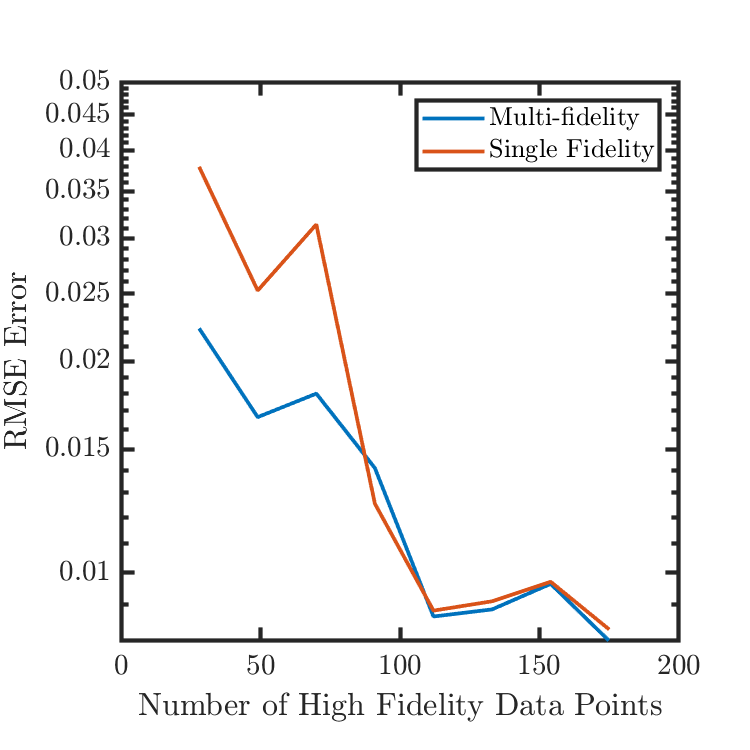
\includegraphics[width=.31\textwidth]{code/image_gen/nasa_crm/suthesis/images/cl_2d_rsme_lhs_comp.png} }
    \end{subfigure}
    \hfill
    \begin{subfigure}[RMSE for $C_D$.]{
        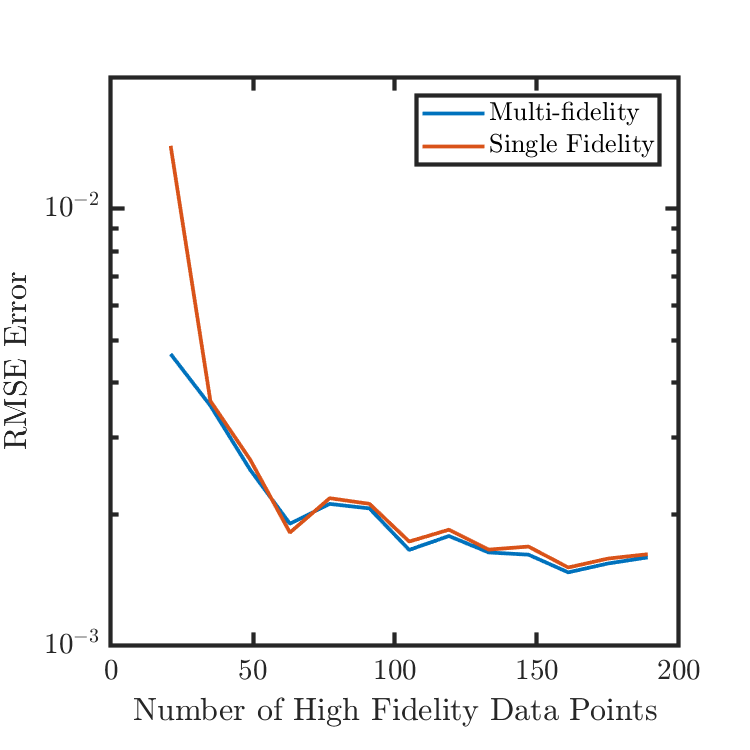
\includegraphics[width=.31\textwidth]{code/image_gen/nasa_crm/suthesis/images/cd_2d_rsme_lhs_comp.png} 
    }
    \end{subfigure}
    \hfill
    \begin{subfigure}[RMSE for $C_m$.]{
        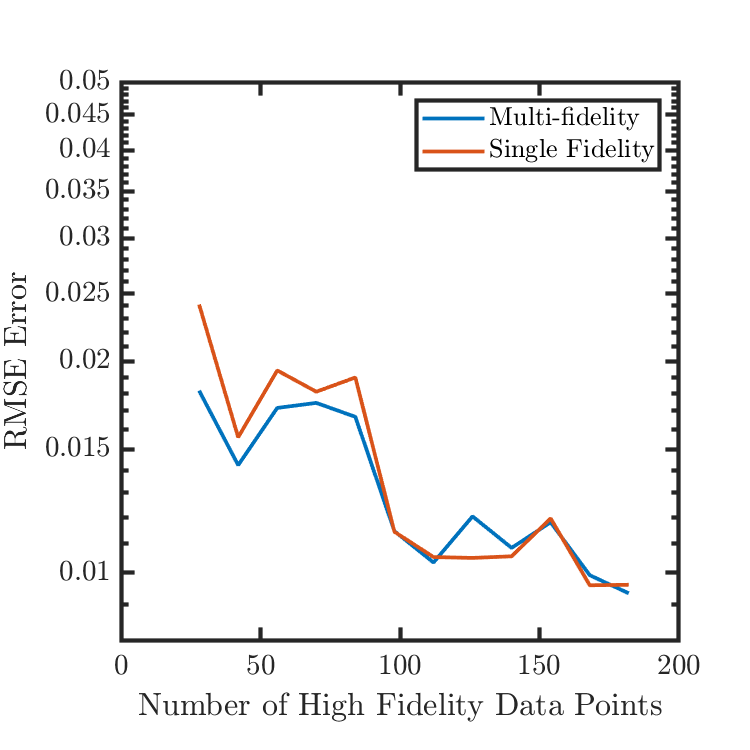
\includegraphics[width=.31\textwidth]{code/image_gen/nasa_crm/suthesis/images/cm_2d_rsme_lhs_comp.png} 
    }
    \end{subfigure}
    \caption{Root-mean-square-error for two-dimensional functions of Mach and $\alpha$ when using two-fidelity data vs. using only high-fidelity data points.\label{fig:2d_mf_vs_hf}}
\end{figure}
